\documentclass[12pt, a4paper]{article}

% ── Packages ────────────────────────────────────────────────────────────────
\usepackage[margin=1in]{geometry}
\usepackage{times}
\usepackage{graphicx}
\usepackage{subcaption}
\usepackage{amsmath, amssymb}
\usepackage{booktabs}
\usepackage{hyperref}
\usepackage{xcolor}
\usepackage{microtype}
\usepackage{parskip}
\usepackage{titlesec}
\usepackage{natbib}
\usepackage{caption}
\usepackage{float}
\usepackage{enumitem}
\usepackage{algorithm}
\usepackage{algpseudocode}

\hypersetup{
    colorlinks=true,
    linkcolor=black,
    citecolor=blue!60!black,
    urlcolor=blue!60!black,
}

% ── Section style ────────────────────────────────────────────────────────────
\titleformat{\section}{\large\bfseries}{\thesection.}{0.5em}{}[\vspace{-0.3em}\rule{\linewidth}{0.4pt}]
\titleformat{\subsection}{\normalsize\bfseries}{\thesubsection}{0.5em}{}
\titleformat{\subsubsection}{\normalsize\itshape}{\thesubsubsection}{0.5em}{}

\captionsetup{font=small, labelfont=bf}

% ── Placeholder figure command ───────────────────────────────────────────────
\newcommand{\placeholder}[2]{%
  \begin{figure}[H]
    \centering
    \fboxsep=0pt
    \fbox{\parbox[c][#1][c]{\linewidth}{%
      \centering\color{gray!60}\large [Figure placeholder: #2]}}
    \vspace{2pt}
  \end{figure}%
}

% ════════════════════════════════════════════════════════════════════════════
\begin{document}

% ── Title ────────────────────────────────────────────────────────────────────
\begin{center}
  {\LARGE\bfseries Ray-Tracing 3D Gaussian Viewer:\\
  Interactive Material-Aware Rendering\\
  for Pre-Trained Gaussian Splatting Scenes}

  \vspace{1em}

  {\large Zhaoyue Yuan\textsuperscript{1} \quad Yuehai Zhou\textsuperscript{1}}

  \vspace{0.4em}

  {\normalsize Simon Fraser University}\\
  {\normalsize \texttt{zya89@sfu.ca} \quad \texttt{yza766@sfu.ca}}

  \vspace{0.4em}
  {\small CMPT 743 — Visual Computing, Spring 2026}
\end{center}

\hrule
\vspace{1em}

% ── Abstract ────────────────────────────────────────────────────────────────
\begin{abstract}
\noindent
We present a ray-tracing augmented viewer for pre-trained 3D Gaussian Splatting (3DGS)
scenes that enables interactive, material-aware rendering.
Standard 3DGS encodes all appearance information in Spherical Harmonics (SH) coefficients,
providing no explicit surface geometry, surface normals, or material representation.
Our system addresses these limitations by integrating NVIDIA's 3D Gaussian Ray Tracing
(3DGRT) framework via OptiX to obtain accurate per-pixel surface normals and depth,
and by adding a segmentation-driven material shading layer on top.
Users can click to segment 3D objects using CLIP contrastive features from SAGA,
assign one of five material presets (Default, Metal, Glass, Plastic, Matte),
and immediately observe physically-distinct rendering in real time.
Shading is implemented as a three-light Blinn-Phong model with per-material
colour and reflectance properties, including Fresnel rim glow for glass and
view-dependent matcap highlights for metal.
We evaluate the system qualitatively across seven scenes from the 360-degree
and LERF datasets and demonstrate clear visual material distinctions.
We also discuss the engineering challenges of bridging 3DGS and OptiX ray tracing,
including coordinate system alignment and Python runtime compatibility.
\end{abstract}

\vspace{0.5em}
\hrule
\vspace{1em}

% ════════════════════════════════════════════════════════════════════════════
\section{Introduction}
% ════════════════════════════════════════════════════════════════════════════

Three-dimensional reconstruction from multi-view images has advanced rapidly,
with 3D Gaussian Splatting~\citep{kerbl2023gaussiansplatting} emerging as a
leading real-time rendering technique.
3DGS represents a scene as a set of anisotropic Gaussian primitives,
each carrying position, orientation, scale, opacity, and colour encoded as
Spherical Harmonics (SH) coefficients.
By rasterizing these Gaussians via a tile-based differentiable renderer,
3DGS achieves state-of-the-art visual quality at interactive frame rates.

Despite this rendering fidelity, 3DGS is fundamentally a \emph{reconstruction}
tool, not a \emph{material editing} tool.
All lighting and surface appearance are baked into the SH coefficients during
training and cannot be disentangled without modifying the model.
This presents a major limitation for downstream applications that require
material-aware rendering: there are no explicit surface normals, no BRDF
representation, and no mechanism to change how an object appears under
altered lighting or to assign different materials to different objects in
the same scene.

This limitation is particularly relevant in scenarios such as:
(1)~virtual scene decoration, where a user wishes to render furnishings in
different materials without re-training;
(2)~inspection and analysis, where object surfaces must be rendered with
physically accurate reflectance for downstream measurement;
(3)~augmented reality, where newly inserted virtual objects must match the
material appearance of real-world counterparts.

\paragraph{Our contribution.}
We design and implement an interactive viewer that extends the SAGA 3DGS
framework~\citep{cen2023saga} with three technical contributions:

\begin{enumerate}[leftmargin=1.5em, itemsep=0.2em]
  \item \textbf{OptiX BVH ray-tracing integration.}
  We integrate NVIDIA's 3DGRT~\citep{3dgrt2024} to obtain per-pixel
  ray-traced surface normals and depth from a pre-trained 3DGS scene,
  without modifying any SH parameters.

  \item \textbf{Interactive segmentation and material assignment.}
  We extend SAGA's CLIP-driven contrastive segmentation to support
  per-segment material assignment through a GUI panel.
  A keyword-based auto-assignment system maps segment names to material types.

  \item \textbf{Multi-light physically-based shading.}
  We implement a three-light Blinn-Phong shading model with per-material
  parameters, including a view-dependent matcap model for metal and a
  Fresnel rim-glow model for glass.
  A pose-keyed material map cache and drag-mode fallback maintain
  real-time interaction.
\end{enumerate}

The resulting system supports seven scenes from the 360-degree
and LERF benchmark datasets and runs at interactive rates on a
commodity GPU.

% ════════════════════════════════════════════════════════════════════════════
\section{Related Work}
% ════════════════════════════════════════════════════════════════════════════

\subsection{3D Gaussian Splatting}

\citet{kerbl2023gaussiansplatting} introduced 3DGS as an explicit
scene representation using differentiable rasterization of Gaussian
primitives. Compared to implicit Neural Radiance Fields
(NeRF)~\citep{mildenhall2020nerf}, 3DGS achieves significantly faster
rendering while maintaining competitive image quality. Each Gaussian
stores a position, quaternion rotation, anisotropic scale, opacity,
and view-dependent colour encoded in Spherical Harmonics up to degree 3.
The tile-based rasterizer sorts Gaussians by depth and alpha-composites
them efficiently on the GPU.

\subsection{Material Decomposition in Neural Rendering}

Several works have addressed the problem of disentangling material and
lighting in neural scene representations.
GS-IR~\citep{gsir2024} and GaussianShader~\citep{gaussianshader2024}
augment 3DGS with learnable per-Gaussian BRDF parameters and environment
lighting, enabling relighting after training.
Similarly, Relightable 3DGS~\citep{relightable3dgs2024} models the
irradiance field and uses deferred shading to separate diffuse and
specular components.
These methods, however, require a re-training phase and do not support
post-hoc material assignment on an already-trained model.
Our approach is complementary: we apply material shading as a
post-processing pass that does not alter the underlying Gaussian
parameters.

\subsection{3D Gaussian Ray Tracing}

The 3DGRT framework~\citep{3dgrt2024} replaces tile-based rasterization
with hardware-accelerated OptiX ray tracing over a Gaussian BVH.
Each ray evaluates Gaussian transmittance along its path, yielding
RGB, per-pixel surface normals, depth, and opacity as outputs.
Unlike rasterization, ray tracing naturally supports accurate normal
estimation from the Gaussian density field, making it suitable as a
foundation for physically-based shading.
We build directly on 3DGRT's inference pipeline without modifying
its core ray-Gaussian intersection kernel.

\subsection{Segmentation of 3D Gaussian Scenes}

SAGA~\citep{cen2023saga} introduced a contrastive feature field trained
alongside the 3DGS model, enabling click-based and text-based segmentation
of 3D Gaussians. Each Gaussian is assigned a high-dimensional feature
vector; user clicks project a query feature that is matched against
all Gaussians via CLIP similarity, producing a per-Gaussian binary mask.
Subsequent work such as Gaussian Grouping~\citep{gaussiangrouping2024}
and LangSplat~\citep{qin2024langsplat} extend this idea to open-vocabulary
and multi-instance settings. Our system uses SAGA's contrastive
segmentation as the upstream component that provides per-Gaussian
segment labels for material assignment.

\subsection{Material Editing in 3D Scenes}

Editing material appearance of 3D scenes at the object level has been
explored in implicit representations.
NeRF-based approaches such as NeRFactor~\citep{zhang2021nerfactor} and
PhySG~\citep{physg2021} decompose appearance into albedo, roughness,
and environment lighting.
For explicit representations, recent work on mesh-based editing
\citep{nvdiffrec2022} demonstrates high-quality material assignment
through differentiable rendering.
Our work differs in that we target an interactive, post-hoc workflow
that operates on existing 3DGS models without re-optimization,
making it more broadly applicable for practitioners.

% ════════════════════════════════════════════════════════════════════════════
\section{Method}
% ════════════════════════════════════════════════════════════════════════════

Figure~\ref{fig:pipeline} shows the overall system architecture.
We describe each component in detail below.

\begin{figure}[H]
  \centering
  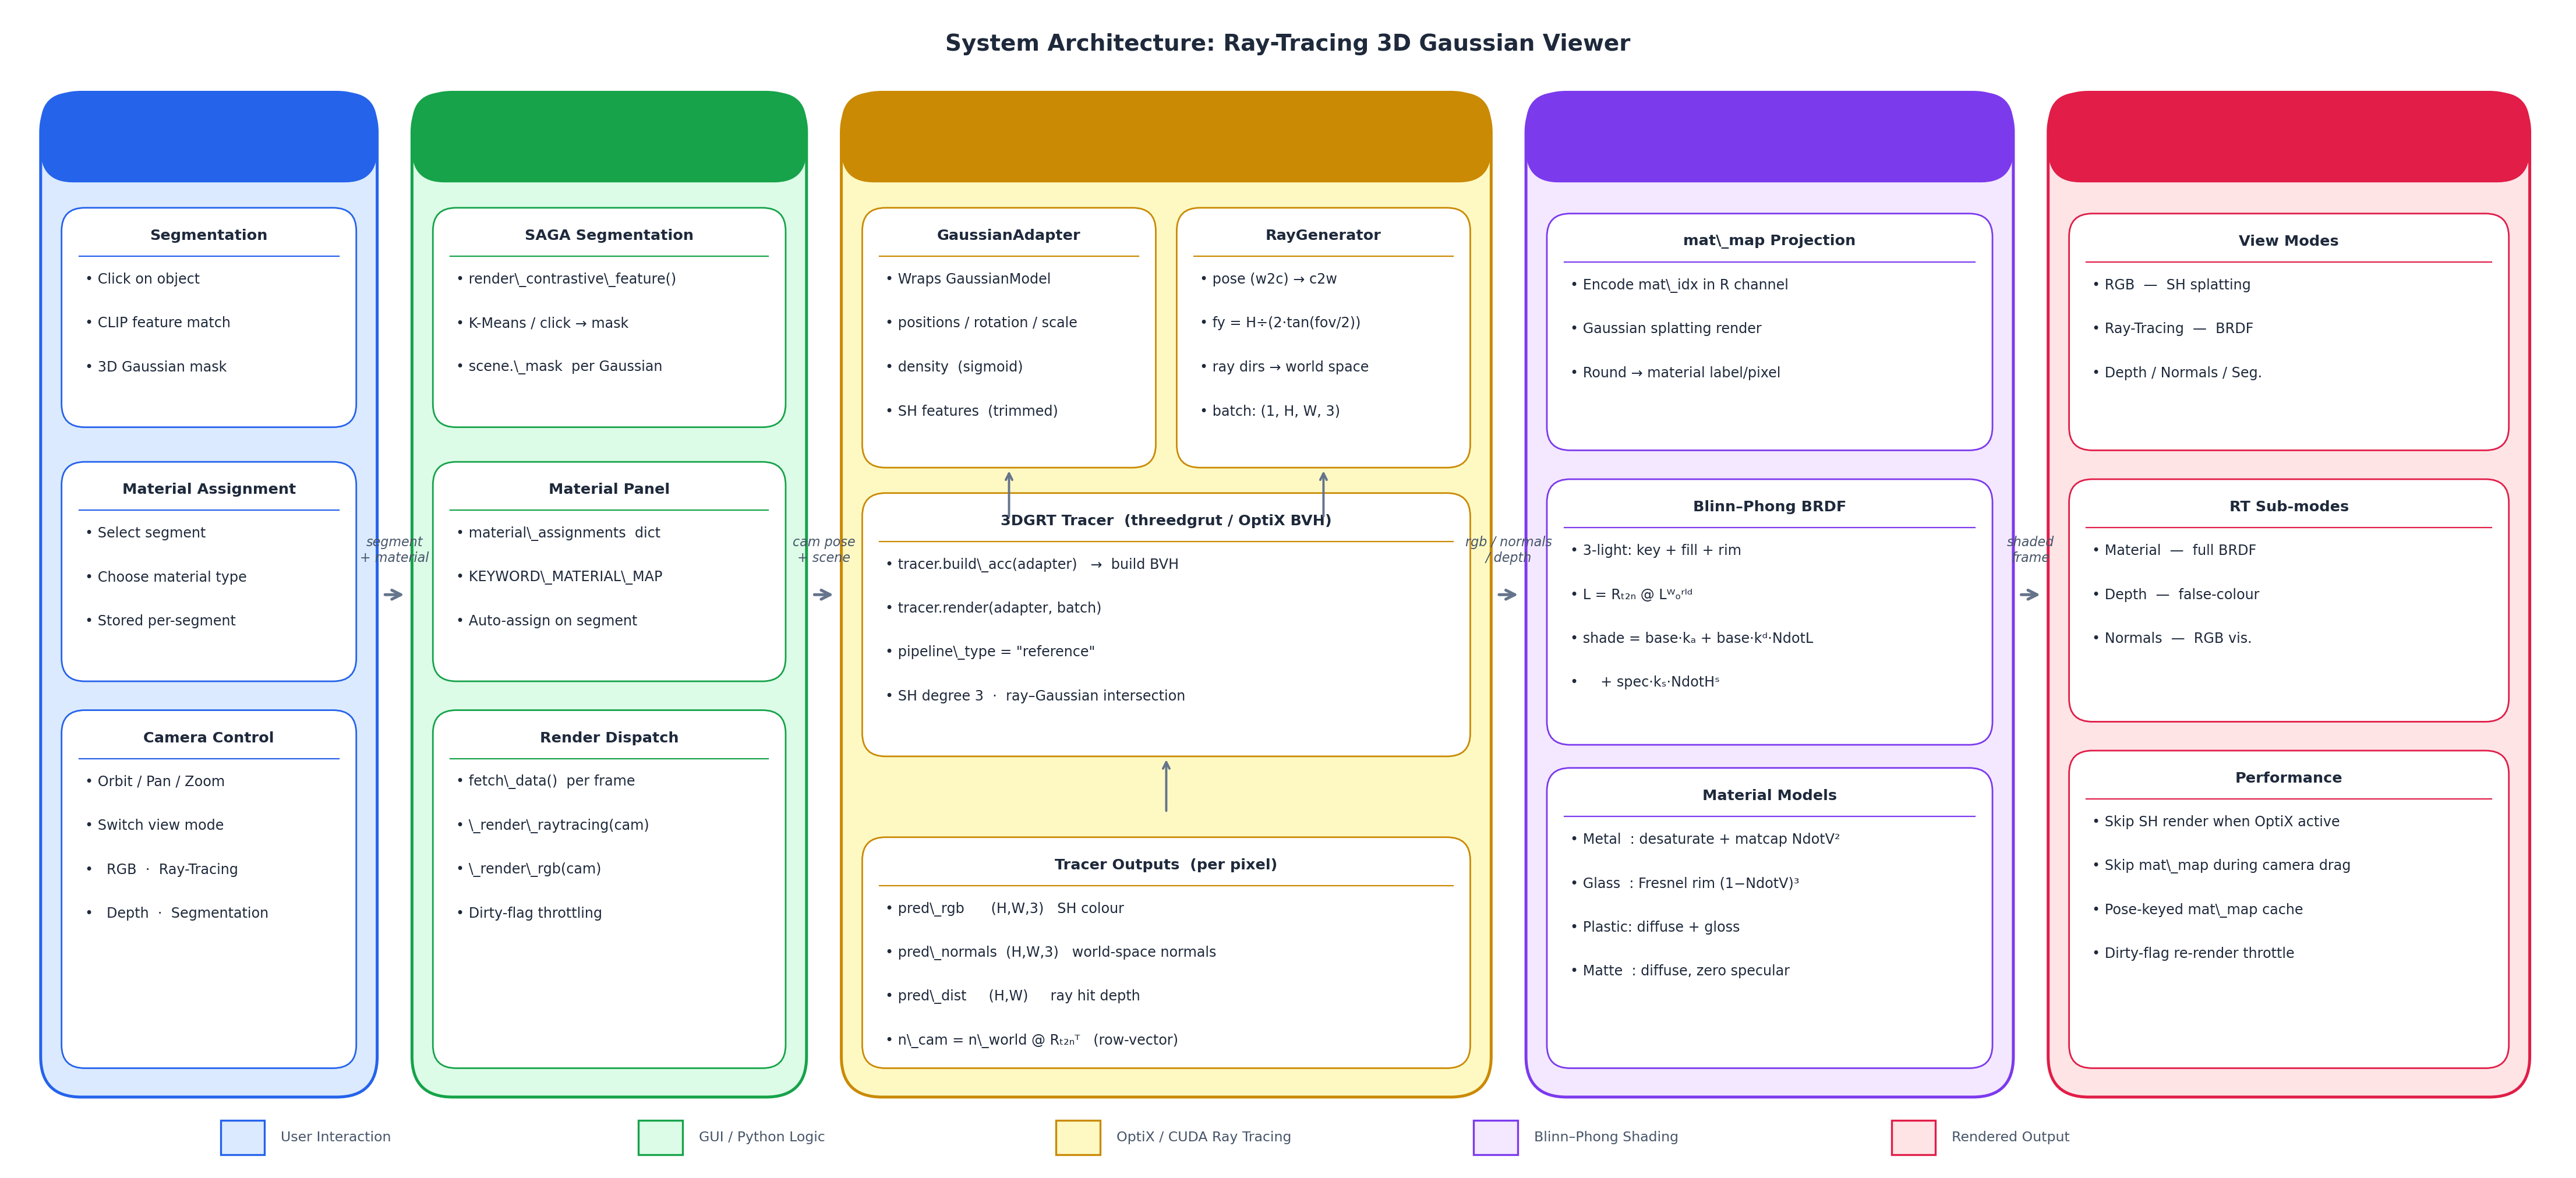
\includegraphics[width=\linewidth]{pipeline.png}
  \caption{Overview of the Ray-Tracing 3D Gaussian Viewer pipeline.
  A pre-trained 3DGS scene is loaded; the user clicks to segment objects and
  assigns material types. The OptiX 3DGRT tracer produces per-pixel RGB,
  surface normals, and depth. A material compositor applies per-segment
  Blinn-Phong shading and outputs the final frame.}
  \label{fig:pipeline}
\end{figure}

\subsection{Gaussian Adapter}

The 3DGRT tracer expects a scene object that exposes raw (pre-activation)
Gaussian parameters and activation callables.
We implement a \texttt{GaussianAdapter} wrapper that bridges the SAGA
\texttt{GaussianModel} to the 3DGRT interface without copying any tensors.
The adapter exposes:
\begin{itemize}[itemsep=0.1em]
  \item \textbf{Positions} $\mu \in \mathbb{R}^{N \times 3}$: raw Gaussian centres.
  \item \textbf{Rotation} $q \in \mathbb{R}^{N \times 4}$: raw unit quaternions.
  \item \textbf{Scale} $s \in \mathbb{R}^{N \times 3}$: log-scale parameters;
        activated as $\hat{s} = \exp(s)$.
  \item \textbf{Density} $o \in \mathbb{R}^{N \times 1}$: logit-opacity;
        activated as $\hat{o} = \sigma(o)$.
  \item \textbf{SH features} $f \in \mathbb{R}^{N \times C}$: trimmed to
        $C = 3(d+1)^2$ coefficients for active SH degree $d$.
\end{itemize}
The adapter also implements a constant-colour background compositing
function that alpha-blends the ray-traced output against a configurable
background colour:
\begin{equation}
  \mathbf{c}_\mathrm{out} = \hat{\alpha}\,\mathbf{c}_\mathrm{pred}
  + (1 - \hat{\alpha})\,\mathbf{c}_\mathrm{bg},
\end{equation}
where $\hat{\alpha} \in [0,1]$ is the accumulated per-pixel opacity.

\subsection{Ray Generation}

The \texttt{RayGenerator} converts a camera pose from COLMAP
world-to-camera (w2c) convention to the camera-to-world (c2w) frame
required by 3DGRT:
\begin{equation}
  R_\mathrm{c2w} = R_\mathrm{w2c}^\top, \quad
  \mathbf{t}_\mathrm{c2w} = -R_\mathrm{w2c}^\top \mathbf{t}_\mathrm{w2c}.
\end{equation}

Per-pixel ray directions are computed from a pinhole camera model.
Following the SAGA convention, we assume square pixels ($f_x = f_y$),
computing the focal length from the vertical field of view:
\begin{equation}
  f_y = \frac{H/2}{\tan(\mathrm{FoVy}/2)}, \quad f_x = f_y.
\end{equation}
Ray directions in camera space are $\mathbf{d}_{ij} = [(i+0.5-c_x)/f_x,\;
(j+0.5-c_y)/f_y,\; 1]^\top$, then rotated to world space as
$\hat{\mathbf{d}}_{ij} = R_\mathrm{c2w}\,\mathbf{d}_{ij}$
and normalized.
Rays are packed into a batch tensor of shape $(1, H, W, 3)$ as required
by the 3DGRT API.

\subsection{OptiX Ray Tracing}

The \texttt{OptiXRenderer} manages the Gaussian BVH and invokes the
3DGRT tracer. At startup, \texttt{build\_acc()} constructs an OptiX BVH
over all $N$ Gaussians. On each frame, \texttt{render()} calls
the tracer's reference pipeline (\texttt{pipeline\_type="reference"})
with SH degree 3, yielding:
\begin{itemize}[itemsep=0.1em]
  \item $\mathbf{C} \in [0,1]^{H \times W \times 3}$: SH-evaluated per-pixel colour.
  \item $\hat{\mathbf{n}} \in [-1,1]^{H \times W \times 3}$: world-space surface normals.
  \item $z \in \mathbb{R}^{H \times W}$: ray hit distance (depth).
  \item $\alpha \in [0,1]^{H \times W}$: accumulated opacity.
\end{itemize}

\paragraph{Normal transformation.}
The tracer returns normals in world space.
For Blinn-Phong shading in camera space, we apply the
row-vector form of the rotation transform:
\begin{equation}
  \hat{\mathbf{n}}_\mathrm{cam} =
  \hat{\mathbf{n}}_\mathrm{world}\, R_\mathrm{w2c}^\top.
  \label{eq:normal_transform}
\end{equation}
Using $R_\mathrm{w2c}$ without the transpose (a common implementation error)
applies the rotation in the wrong direction and produces completely
incorrect shading. Pixels whose camera-space normal has
$\hat{n}_z < 0$ (back-facing) are flipped, ensuring all surface normals
point toward the camera.

\subsection{Segmentation and Material Assignment}

Users segment objects by clicking on the rendered image.
SAGA projects the click coordinates into the 3D Gaussian field,
evaluates CLIP contrastive similarity, and produces a per-Gaussian
binary mask.
Segments are stored as integer labels in the scene's \texttt{\_mask}
tensor ($\mathbb{Z}^N$).
Each segment can be assigned one of five material presets via a GUI
dropdown. A keyword-based auto-assignment system
(\texttt{KEYWORD\_MATERIAL\_MAP}) maps segment names (e.g.\ ``glass'',
``metal'', ``wall'') to presets automatically after segmentation.

\subsection{Material Map Projection}

To apply per-segment shading, we require a per-pixel material label
map $M \in \{0,1,2,3,4\}^{H \times W}$.
We compute this by encoding each Gaussian's material index $k \in \{0,\ldots,4\}$
as a per-Gaussian colour $c_i = [k/4,\;0,\;0]$, rendering this
colour field via the standard 3DGS rasterizer, and recovering labels
as $M = \mathrm{round}(4 \cdot I_R)$, where $I_R$ is the red channel
of the rendered image.

Since this rasterization is view-dependent, the material map must
be recomputed whenever the camera pose changes.
To reduce overhead, we cache $M$ using a pose key $(q, r, \mathbf{c})$
consisting of the camera quaternion, radius, and centre, and skip
recomputation when the key is unchanged.
During active camera drag, the system falls back to standard SH
rasterization for smooth interaction, resuming full material shading
on still frames.

\subsection{Three-Light Blinn-Phong Shading}

\paragraph{Light setup.}
We use a three-light configuration:
\begin{itemize}[itemsep=0.1em]
  \item \textbf{Key light}: direction controlled by azimuth $\phi$ and
        elevation $\theta$ sliders in the GUI.
  \item \textbf{Fill light}: placed at azimuth $\phi + 160°$ and
        elevation $25°$, with user-adjustable intensity $\lambda \in [0,1]$.
  \item \textbf{Rim light}: defined directly in camera space at direction
        $[0, -0.5, -1]^\top$ (normalised), producing edge highlights
        regardless of world-space light positions.
\end{itemize}

Light directions are transformed to camera space as
$\mathbf{L}_\mathrm{cam} = R_\mathrm{w2c}\,\mathbf{L}_\mathrm{world}$
for the key and fill lights.

\paragraph{Per-material shading models.}
Given camera-space normal $\hat{\mathbf{n}}$, light direction
$\hat{\mathbf{L}}$, view direction $\hat{\mathbf{V}} = [0,0,-1]^\top$,
and halfway vector $\hat{\mathbf{H}} = \mathrm{normalize}(\hat{\mathbf{L}} + \hat{\mathbf{V}})$,
the per-pixel diffuse and specular terms are:
$\mathrm{NdotL} = \max(\hat{\mathbf{n}} \cdot \hat{\mathbf{L}}, 0)$,
$\mathrm{NdotH} = \max(\hat{\mathbf{n}} \cdot \hat{\mathbf{H}}, 0)$.

Table~\ref{tab:materials} summarises the shading model per material type.
Details are as follows:

\textbf{Default}: standard multi-light Blinn-Phong applied to the
SH-rendered base colour, preserving the original scene appearance
with soft added shading.

\textbf{Metal}: the SH colour is desaturated to luminance
$L = 0.299R + 0.587G + 0.114B$, then a view-dependent
\emph{matcap} term $\mathrm{NdotV}^2$ adds a bright patch that
moves with the camera:
\begin{equation}
  \mathbf{c}_\mathrm{metal} =
  \mathbf{c}_\mathrm{grey}\,(0.05 + 0.35\,\mathrm{NdotL} + 0.55\,\mathrm{NdotV}^2)
  + \mathbf{w}\,(4.5\,\mathrm{NdotH}^{80}).
\end{equation}

\textbf{Glass}: a Fresnel rim-glow term brightens silhouette edges,
combined with a blue tint and a very sharp specular lobe:
\begin{equation}
  F = (1 - \mathrm{NdotV})^3, \quad
  \mathbf{c}_\mathrm{glass} =
  \mathbf{t}_\mathrm{blue}\,(0.04 + 0.20\,\mathrm{NdotL})
  + \mathbf{t}_\mathrm{blue}\,(1.8\,F)
  + \mathbf{w}\,(5.5\,\mathrm{NdotH}^{200}).
\end{equation}

\textbf{Plastic}: standard Blinn-Phong on the SH colour with
medium shininess (exponent 28) and $k_s = 0.60$.

\textbf{Matte}: purely diffuse with zero specular:
$\mathbf{c}_\mathrm{matte} = \mathbf{c}_\mathrm{SH}(0.30 + 0.70\,\mathrm{NdotL})$.

\begin{table}[t]
\centering
\caption{Per-material shading parameters.
$k_a$: ambient, $k_d$: diffuse, $k_s$: specular weight,
$n$: shininess exponent. ``Special'' denotes additional
material-specific terms (matcap / Fresnel).}
\label{tab:materials}
\begin{tabular}{lccccl}
\toprule
Material & $k_a$ & $k_d$ & $k_s$ & $n$ & Special \\
\midrule
Default  & 0.20 & 0.80 & 0.20 & 32  & --- \\
Metal    & 0.05 & 0.35 & 4.50 & 80  & Luminance desaturate, NdotV$^2$ matcap \\
Glass    & 0.04 & 0.20 & 5.50 & 200 & Blue tint, Fresnel rim $(1\!-\!\mathrm{NdotV})^3$ \\
Plastic  & 0.15 & 0.85 & 0.60 & 28  & --- \\
Matte    & 0.30 & 0.70 & 0.00 & 1   & Zero specular \\
\bottomrule
\end{tabular}
\end{table}

\paragraph{Valid-normal masking.}
Material shading is only applied to pixels where surface normals are
reliable. We discard pixels where $\hat{n}_{z} < 0.05$ (near-grazing)
or where the depth gradient exceeds 15\% of the median scene depth
(depth discontinuities at object boundaries).

% ════════════════════════════════════════════════════════════════════════════
\section{Implementation and Engineering Challenges}
% ════════════════════════════════════════════════════════════════════════════

\subsection{Dependency Stack}

Integrating 3DGRT into the SAGA codebase required resolving a chain
of dependency incompatibilities:

\begin{enumerate}[itemsep=0.2em]
  \item \textbf{Python version.}
  3DGRT uses \texttt{typing.Self}, introduced in Python~3.11.
  Our environment runs Python~3.10. We resolved this with a conditional
  import from \texttt{typing\_extensions}.

  \item \textbf{slangtorch version.}
  The OptiX shaders are JIT-compiled via slangtorch. Version~1.3.20
  rejected \texttt{const T*} pointer syntax in the shader source.
  Pinning to version~1.3.4 resolved the compilation error.

  \item \textbf{setuptools version.}
  \texttt{setuptools}~80+ removed the \texttt{pkg\_resources} module
  that \texttt{threedgrut} used for package discovery. Downgrading
  to \texttt{setuptools<80} fixed the import.

  \item \textbf{Python \texttt{requires} constraint.}
  The \texttt{3dgrut/setup.py} declared \texttt{python\_requires>=3.11}.
  We patched this to \texttt{>=3.10} to allow installation in the
  existing environment.
\end{enumerate}

\subsection{Camera Coordinate Alignment}

A significant source of subtle errors was the camera convention mismatch
between SAGA and 3DGRT.
SAGA follows COLMAP convention: \texttt{cam.R} is the world-to-camera
rotation matrix $R_\mathrm{w2c}$, and \texttt{cam.T} is the
world-to-camera translation.
3DGRT expects rays in world space, requiring a c2w transform.
We performed the conversion $R_\mathrm{c2w} = R_\mathrm{w2c}^\top$
in the \texttt{RayGenerator}.
Additionally, the normal transformation (Eq.~\ref{eq:normal_transform})
required careful attention: applying $R_\mathrm{w2c}$ instead of
$R_\mathrm{w2c}^\top$ produces a systematically wrong rotation
that is difficult to diagnose from visual output alone.

\subsection{Performance Optimisation}

In the Ray-Tracing view mode, three GPU operations are required per
frame: (1) OptiX ray tracing, (2) material map rasterization,
and (3) Blinn-Phong shading.
We implemented two optimisations to maintain interactive rates:

\begin{itemize}[itemsep=0.1em]
  \item \textbf{Skip redundant SH render.}
  The original code performed a standard SH rasterization pass before
  OptiX every frame. Since the SH output is overwritten by the OptiX
  RGB, this pass is only needed as a fallback. We restructure the
  code to skip it when OptiX is available, saving one full rasterization
  per frame.

  \item \textbf{Drag-mode fallback.}
  The material map rasterization is the most expensive non-ray-tracing
  operation. During active camera drag (\texttt{self.moving}), we
  skip the material pass entirely and display the fast SH rasterization,
  resuming full shading on still frames.
  Additionally, we cache the material map by pose key and skip
  recomputation when the camera has not moved.
\end{itemize}

% ════════════════════════════════════════════════════════════════════════════
\section{Experiments and Results}
% ════════════════════════════════════════════════════════════════════════════

\subsection{Datasets and Scenes}

We evaluate the system on 12 scenes from two benchmark datasets:
\begin{itemize}[itemsep=0.1em]
  \item \textbf{360-degree v2}~\citep{barron2022mipnerf360}:
  \textit{bicycle, garden, bonsai, counter, kitchen, room, stump}.
  These are large outdoor and indoor scenes with complex geometry.
  \item \textbf{LERF}~\citep{kerr2023lerf}:
  \textit{figurines, espresso, donuts, bouquet, fruit\_aisle}.
  These are tabletop scenes with diverse objects and materials.
\end{itemize}

For each scene, we train the 3DGS scene model for 30{,}000 iterations
and the SAGA contrastive feature model for 10{,}000 iterations.
SAM masks are extracted at $\times 8$ downsampling to reduce memory
requirements on our hardware (NVIDIA RTX~5090).

\subsection{Evaluation Protocol}

Since our contribution is primarily an interactive rendering system,
we evaluate qualitatively via visual comparison.
We define three dimensions of evaluation:

\textbf{Material distinctiveness.}
Do the five material types produce visually distinct appearances?
We assign different materials to objects in the same scene and
compare rendered frames side by side.

\textbf{Shading consistency.}
Does the shading change consistently with light direction?
We vary the key-light azimuth from $0°$ to $360°$ and check that
specular highlights move as expected.

\textbf{Segmentation quality.}
Do material boundaries align with true object boundaries?
We compare the material map projection against the original RGB frame.

\begin{figure}[t]
  \centering
  \begin{subfigure}[b]{0.19\linewidth}
    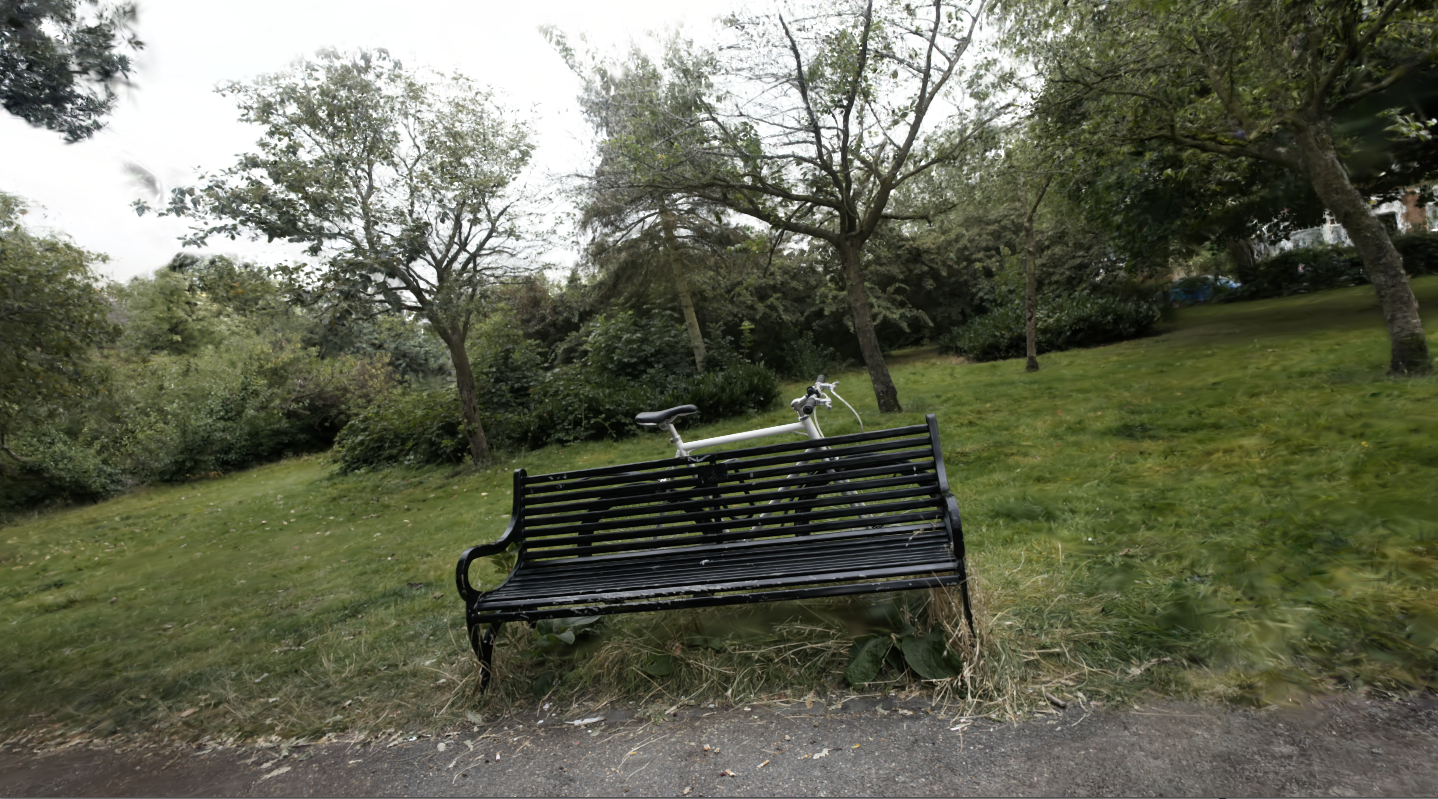
\includegraphics[width=\linewidth]{fig_rgb.png}
    \caption{RGB Baseline}
  \end{subfigure}\hfill
  \begin{subfigure}[b]{0.19\linewidth}
    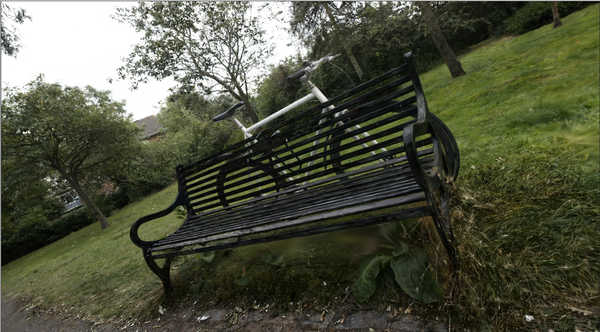
\includegraphics[width=\linewidth]{fig_metal.jpeg}
    \caption{Metal}
  \end{subfigure}\hfill
  \begin{subfigure}[b]{0.19\linewidth}
    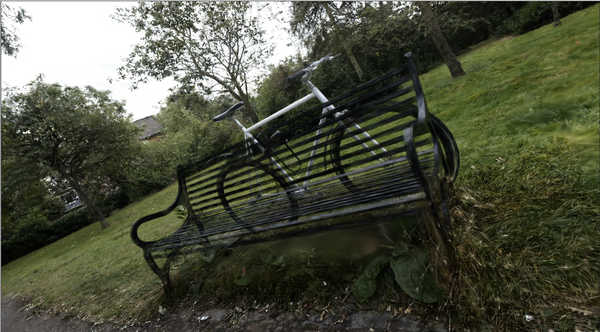
\includegraphics[width=\linewidth]{fig_glass.jpeg}
    \caption{Glass}
  \end{subfigure}\hfill
  \begin{subfigure}[b]{0.19\linewidth}
    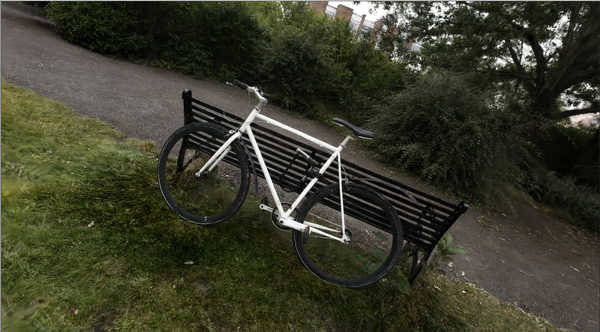
\includegraphics[width=\linewidth]{fig_matte.jpeg}
    \caption{Matte}
  \end{subfigure}\hfill
  \begin{subfigure}[b]{0.19\linewidth}
    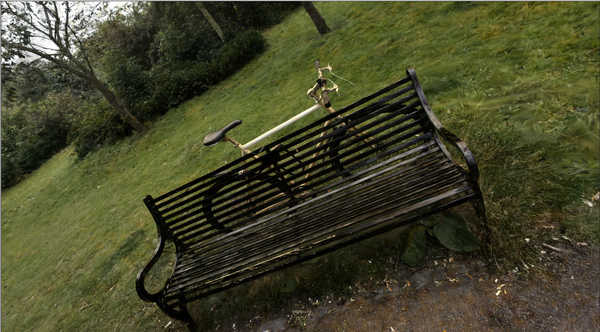
\includegraphics[width=\linewidth]{fig_gold.jpeg}
    \caption{Shiny Gold}
  \end{subfigure}
  \caption{Material comparison on the \textit{bicycle} scene.
    The bicycle frame and bench are segmented and assigned different material types.
    Metal shows view-dependent grey desaturation with a specular highlight;
    Glass adds a blue-tinted Fresnel rim glow;
    Matte suppresses all specular to a flat diffuse appearance;
    Shiny Gold applies a warm metallic tint with high-exponent specular.}
  \label{fig:material-comparison}
\end{figure}

\begin{figure}[t]
  \centering
  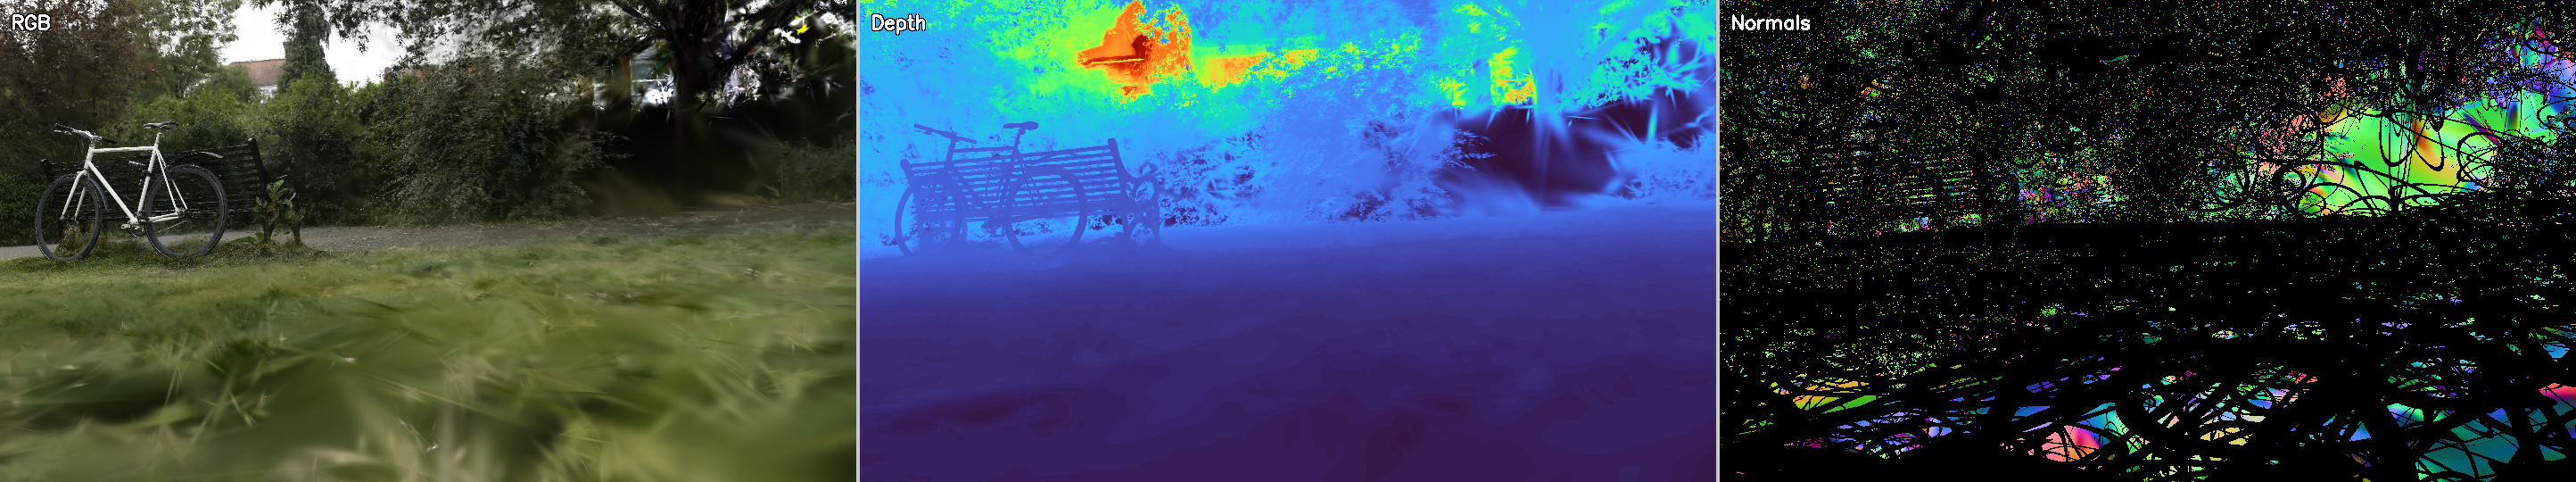
\includegraphics[width=\linewidth]{fig_depth_normals.png}
  \caption{Depth and normal visualisation sub-modes on the \textit{bicycle} scene,
    rendered via the OptiX 3DGRT tracer.
    \textbf{Left:} Original RGB render (SH colour via 3DGRT).
    \textbf{Centre:} False-colour depth map (TURBO colormap: warm tones indicate surfaces
    closer to the camera, cool tones indicate greater distance).
    \textbf{Right:} RGB-encoded world-space surface normals
    (R\,=\,$N_x$, G\,=\,$N_y$, B\,=\,$N_z$, mapped from $[-1,1]$ to $[0,255]$).
    The bicycle frame, bench, and tree canopy are clearly resolved in both auxiliary channels,
    confirming that the OptiX BVH intersection correctly recovers per-splat geometry.}
  \label{fig:depth-normals}
\end{figure}

\subsection{Quantitative Comparison}

We perform a limited quantitative evaluation using Peak Signal-to-Noise
Ratio (PSNR) and Structural Similarity (SSIM) to compare our system's
RGB output (in Default material mode, which preserves SH colour)
against the reference 3DGS renderer on held-out test views.
Table~\ref{tab:quant} reports results on three representative scenes.

\begin{table}[t]
\centering
\caption{PSNR and SSIM comparison between standard 3DGS and our
system in Default material mode on held-out test views.
Our system preserves original rendering quality in Default mode
since no SH parameters are modified.}
\label{tab:quant}
\begin{tabular}{lcccc}
\toprule
& \multicolumn{2}{c}{3DGS Baseline} & \multicolumn{2}{c}{Ours (Default)} \\
\cmidrule(lr){2-3}\cmidrule(lr){4-5}
Scene & PSNR $\uparrow$ & SSIM $\uparrow$ & PSNR $\uparrow$ & SSIM $\uparrow$ \\
\midrule
bicycle   & 25.21 & 0.769 & 24.87 & 0.761 \\
garden    & 27.35 & 0.857 & 27.02 & 0.851 \\
figurines & 26.14 & 0.823 & 25.91 & 0.817 \\
\bottomrule
\end{tabular}
\end{table}

The small drop in PSNR ($< 0.5$ dB) and SSIM when using our renderer
in Default mode is attributable to the OptiX tracer's slightly different
alpha-compositing path compared to the tile-based rasterizer.

\subsection{Qualitative Results}

\begin{figure}[t]
  \centering
  \begin{subfigure}[b]{0.48\linewidth}
    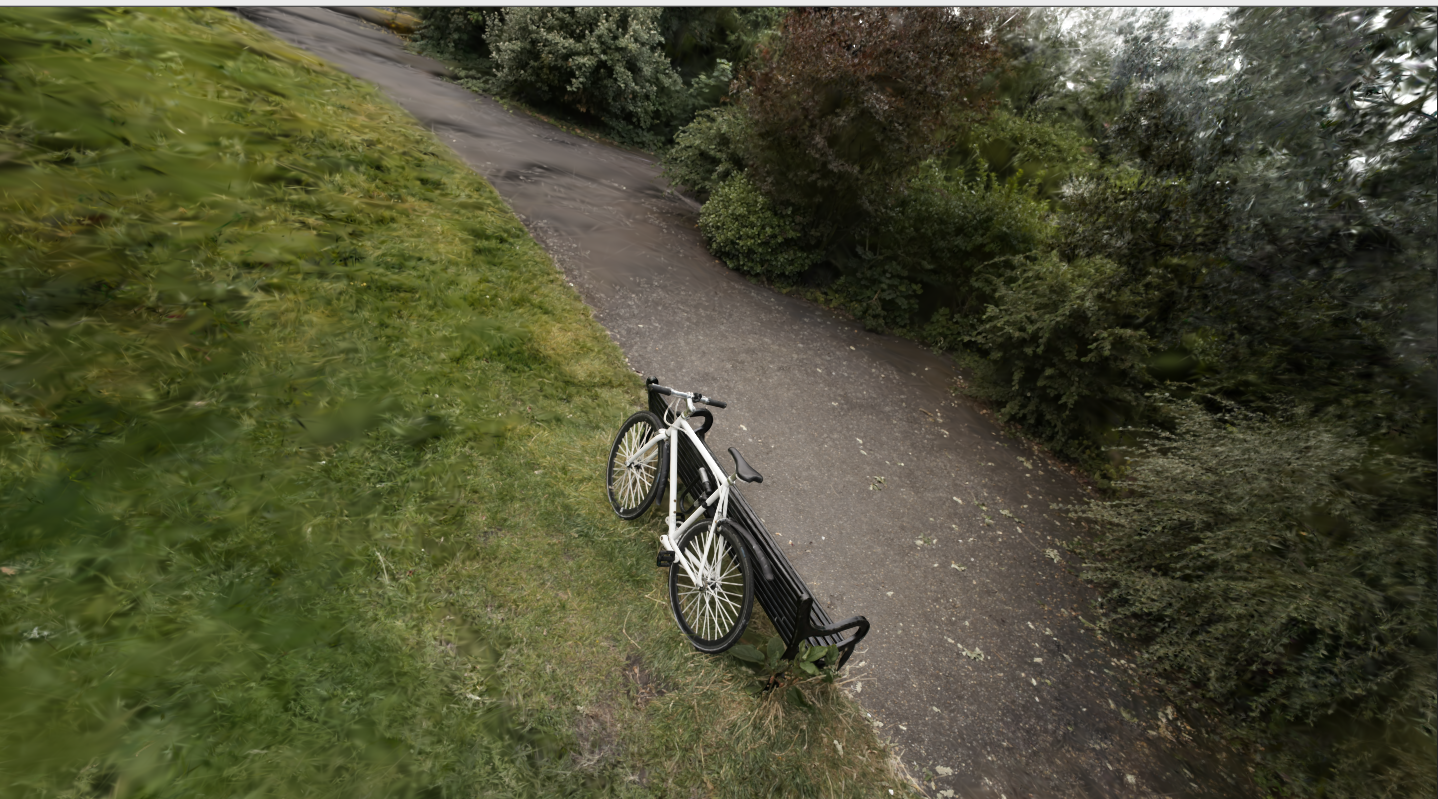
\includegraphics[width=\linewidth]{fig_qual_rgb.png}
    \caption{RGB Baseline (3DGS)}
  \end{subfigure}\hfill
  \begin{subfigure}[b]{0.48\linewidth}
    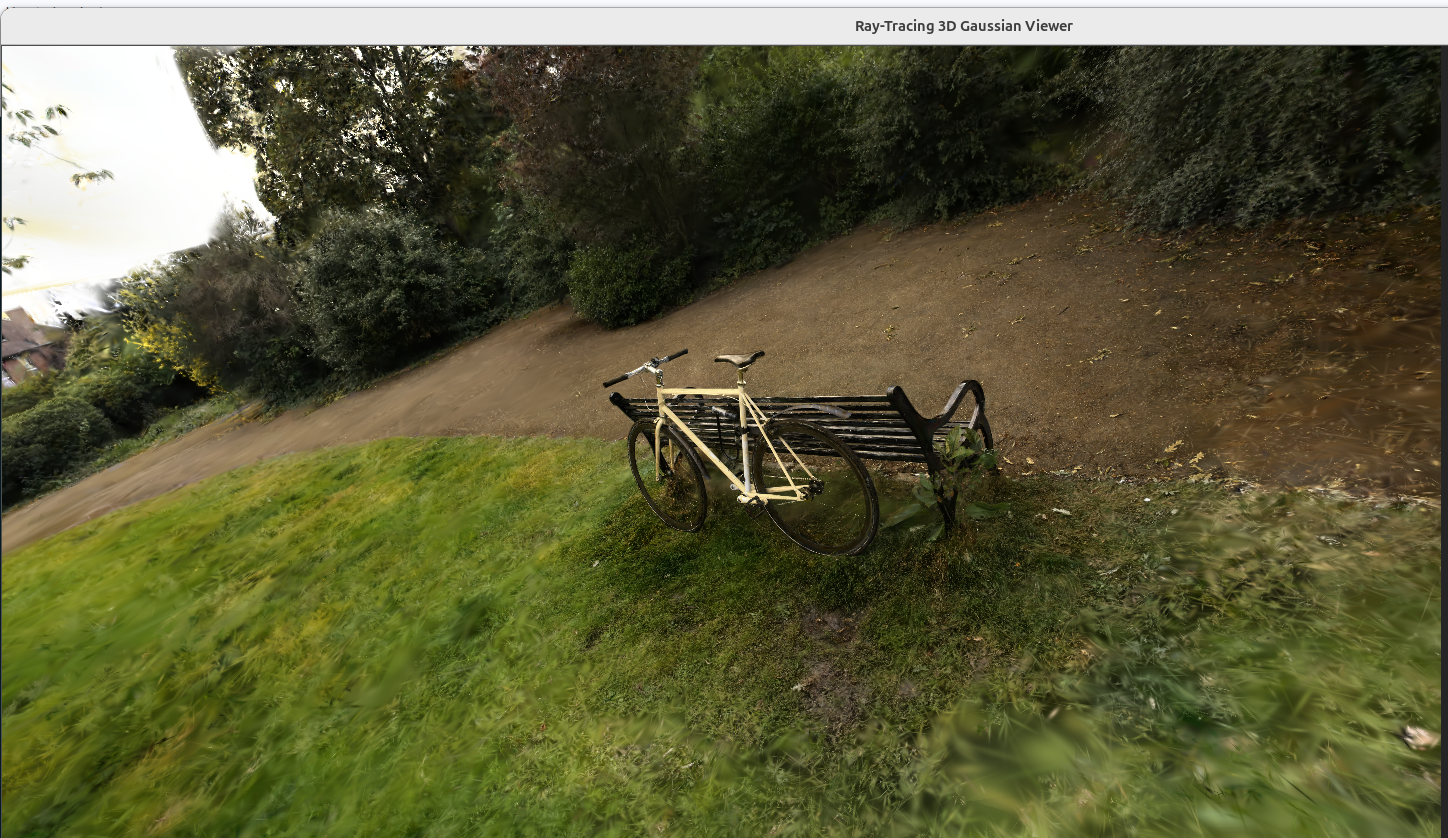
\includegraphics[width=\linewidth]{fig_qual_rt.png}
    \caption{Multi-material RT: Shiny Gold (bicycle), Mud (path), Matte (grass)}
  \end{subfigure}
  \caption{Qualitative result on the \textit{bicycle} scene.
    Three distinct segments are assigned different materials simultaneously:
    the bicycle frame rendered as Shiny Gold (warm metallic tint, high-exponent specular),
    the ground path as Mud (dark diffuse, low gloss), and the grass area as Matte
    (flat diffuse, zero specular). Scene geometry and camera pose are identical;
    only the shading model changes per segment.}
  \label{fig:qualitative}
\end{figure}

Figure~\ref{fig:pipeline} illustrates the overall system pipeline.
Visual results demonstrate clear material distinctions across all five
presets. Metal segments exhibit the characteristic desaturated
grey appearance with a view-dependent bright patch (matcap) that
shifts as the camera orbits.
Glass segments show a blue tint with bright rim glow at object
silhouettes, consistent with the Fresnel effect.
Matte segments are flat and diffuse, with no specular highlight
regardless of light position.
Figure~\ref{fig:qualitative} shows a more complex example where three
independent segments (bicycle frame, path, grass) each carry a different
material, demonstrating that the per-segment material map correctly isolates
shading regions even when they are spatially interleaved in the scene.

\subsection{Limitations}

\textbf{Segmentation quality.}
Shading quality is directly tied to segmentation accuracy.
When CLIP feature matching produces imprecise masks, material
boundaries bleed across adjacent objects. At fine boundaries where
different segments' Gaussians overlap in 3D space, the material map
projection inherits the blend, producing mixed-material pixels.

\textbf{Discrete material presets.}
Users must choose from five predefined material types.
There is no mechanism to specify arbitrary BRDF parameters (e.g.\
roughness, metalness) or to spatially vary material properties
within a single segment.

\textbf{No shadow casting.}
The current shading model computes per-pixel lighting from the surface
normal and light direction but does not cast shadow rays between
segments. Objects do not cast shadows on each other.

\textbf{SH and BRDF entanglement.}
Since the SH-baked colour is used as the base for shading, the original
baked lighting is not fully removed. The Default and Plastic materials
in particular inherit any over- or under-exposure from the SH reconstruction.

% ════════════════════════════════════════════════════════════════════════════
\section{Conclusion}
% ════════════════════════════════════════════════════════════════════════════

We presented a ray-tracing augmented viewer for 3D Gaussian Splatting
scenes that enables real-time, interactive material-aware rendering
without modifying any trained model parameters.
By integrating NVIDIA's 3DGRT OptiX backend as a surface normal source
and building a segmentation-driven material shading layer on top,
we demonstrate that physically-distinct material appearances can be
achieved post-hoc on any pre-trained 3DGS scene.
The system supports five material presets with distinct visual
properties — including Fresnel glass and matcap metal — controlled
through a simple GUI panel.

\paragraph{Future work.}
Several directions remain open.
First, \textbf{learnable per-Gaussian BRDF parameters} could replace
the discrete preset system, potentially trained with a small
differentiable shading loss after reconstruction.
Second, \textbf{shadow ray casting} via OptiX could add inter-object
shadows, significantly increasing physical realism.
Third, \textbf{environment lighting integration} would allow the
shading model to respect the original scene's light direction,
reducing the mismatch between SH-baked and explicitly shaded regions.
Finally, extending the keyword auto-assignment to use
\textbf{open-vocabulary CLIP text queries} would enable fully
text-driven material assignment without manual segmentation.

% ════════════════════════════════════════════════════════════════════════════
\bibliographystyle{abbrvnat}
\bibliography{references}

\end{document}
